
\documentclass{beamer}
\usecolortheme{dove}
\setbeamertemplate{navigation symbols}{}
\usepackage{amsmath,amssymb,amsfonts,amsthm, multicol, subfigure, color}
\usepackage{bm}
\usepackage{graphicx}
\usepackage{tabularx}
\usepackage{booktabs}
\usepackage{hyperref}
\usepackage{pdfpages}
\usepackage{xcolor}
\definecolor{seagreen}{RGB}{46, 139, 87}
\definecolor{mustard}{RGB}{234, 170, 0}
\def\independenT#1#2{\mathrel{\rlap{$#1#2$}\mkern2mu{#1#2}}}
\newcommand\indep{\protect\mathpalette{\protect\independenT}{\perp}}
\def\log{\text{log}}
\newcommand\logit{\text{logit}}
\newcommand\iid{\stackrel{\text{iid}}{\sim}}
\newcommand\E{\text{E}}
\newcommand\V{\text{V}}
\renewcommand\P{\text{P}}
\newcommand{\Cov}{\text{Cov}}
\newcommand{\Cor}{\text{Cor}}
\newcommand\doop{\texttt{do}}
\usepackage{stackrel}
\usepackage{tikz}
\usetikzlibrary{arrows,shapes.arrows,positioning,shapes,patterns,calc}
\newcommand\slideref[1]{\vskip .1cm \tiny \textcolor{gray}{{#1}}}
\newcommand\red[1]{\color{red}#1}
\newcommand\blue[1]{\color{blue}#1}
\newcommand\gray[1]{\color{gray}#1}
\newcommand\seagreen[1]{\color{seagreen}#1}
\newcommand\purple[1]{\color{purple}#1}
\newcommand\orange[1]{\color{orange}#1}
\newcommand\black[1]{\color{black}#1}
\newcommand\white[1]{\color{white}#1}
\newcommand\teal[1]{\color{teal}#1}
\newcommand\magenta[1]{\color{magenta}#1}
\newcommand\Fuchsia[1]{\color{Fuchsia}#1}
\newcommand\BlueGreen[1]{\color{BlueGreen}#1}
\newcommand\bblue[1]{\textcolor{blue}{\textbf{#1}}}
\newcommand\bred[1]{\textcolor{red}{\textbf{#1}}}
\newcommand\bgray[1]{\textcolor{gray}{\textbf{#1}}}
\newcommand\bgreen[1]{\textcolor{seagreen}{\textbf{#1}}}
\newcommand\bref[2]{\href{#1}{\color{blue}{#2}}}
\colorlet{lightgray}{gray!40}
\pgfdeclarelayer{bg}    % declare background layer for tikz
\pgfsetlayers{bg,main} % order layers for tikz
\newcommand\mycite[1]{\begin{scriptsize}\textcolor{darkgray}{(#1)}\end{scriptsize}}
\newcommand{\tcframe}{\frame{
%\small{
\only<1|handout:0>{\tableofcontents}
\only<2|handout:1>{\tableofcontents[currentsubsection]}}
%}
}

\newcommand{\goalsframe}{\begin{frame}{Learning goals for today}
By the end of class, you will be able to
\begin{itemize}
    \item engage with the concepts of social hierarchy beyond income
    \begin{itemize}
    \item social class as ownership of capital
    \item social class as authority and skills
    \item cultural capital
    \item status hierarchies
    \end{itemize}
    \item connect these ideas to data sources
\end{itemize} \vskip .2in
\end{frame}}

\usepackage[round]{natbib}
\bibliographystyle{humannat-mod}
\setbeamertemplate{enumerate items}[default]
\usepackage{mathtools}

\title{Studying Social Inequality with Data Science}
\author{Ian Lundberg}
\date{\today}

\begin{document}

\begin{frame}
\begin{tikzpicture}[x = \textwidth, y = \textheight]
\node at (0,0) {};
\node at (1,1) {};
\node[anchor = north west, align = left, font = \huge] at (0,.9) {Studying\\Social Inequality\\with Data Science};
\node[anchor = north east, align = right] (number) at (1,.9) {INFO 3370 / 5371\\Spring 2023};
\node[anchor = north, font = \Large, align = right] at (.5,.5) {\bblue{Social Class}};
\end{tikzpicture}
\end{frame}

\goalsframe

\begin{frame}{Discussion recap}

If you were asked to use one of four names for your social class, which would you say you belong in: the lower class, the working class, the middle class, or the upper class? \vskip .2in

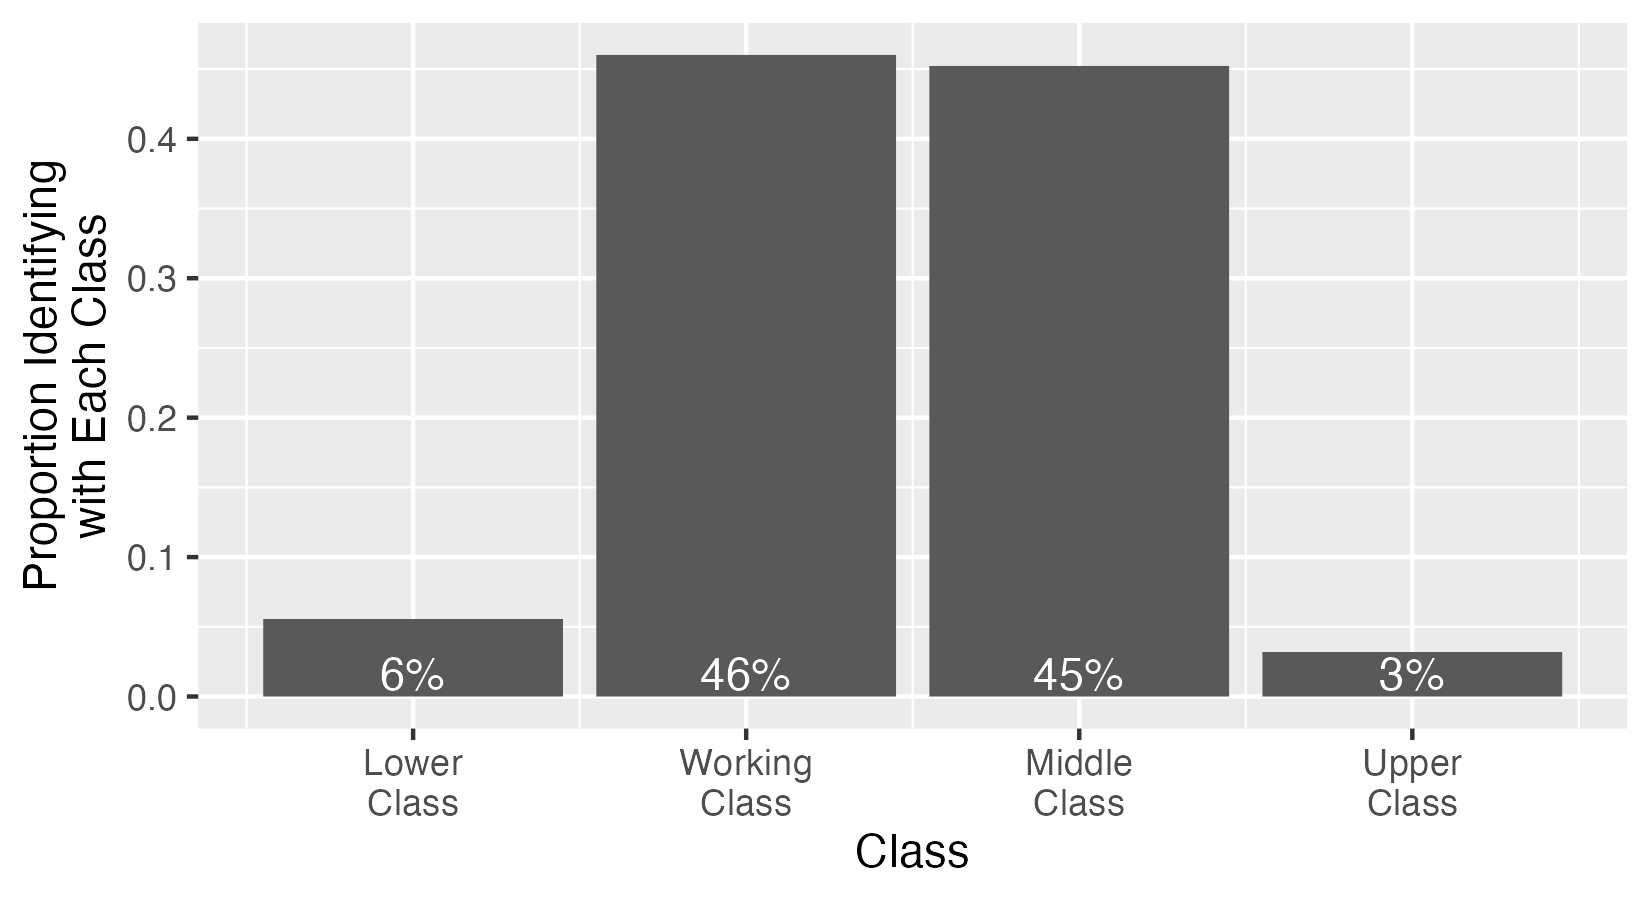
\includegraphics[width = .9\textwidth]{class}

\end{frame}

\begin{frame}

\begin{enumerate}
\item Should we study social class?
\item If so, how would you define it?
\end{enumerate}

\end{frame}

\begin{frame}{Class as ownership of capital}{A Marxist view}

\begin{itemize}
\item capital creates a system of power relations \pause
\item classes are in \textbf{conflict}
\begin{enumerate} \pause
\item some own the means of production \pause
\item some can only sell their labor to (1)
\end{enumerate} \pause
\item capitalists \textbf{exploit} the laborers
\begin{itemize} \pause
\item how much does the capitalist pay to a laborer? \pause
\item only enough for the laborer to eat and survive \pause
\item capitalist keeps all the profit
\end{itemize}
\end{itemize} \vskip .2in \pause
How do we see this today?

\end{frame}

\begin{frame}{Class as ownership of capital}
A data science project could \pause
\begin{itemize}
\item describe stock market returns that exceed growth \pause
\item describe home values that rise faster than inflation \pause
\item describe the consolidation of capital in fewer hands
\end{itemize}
\end{frame}

\begin{frame}{Class as ownership of capital}{\bref{https://www.pewresearch.org/social-trends/2020/01/09/trends-in-income-and-wealth-inequality/}{Pew Research Center}}

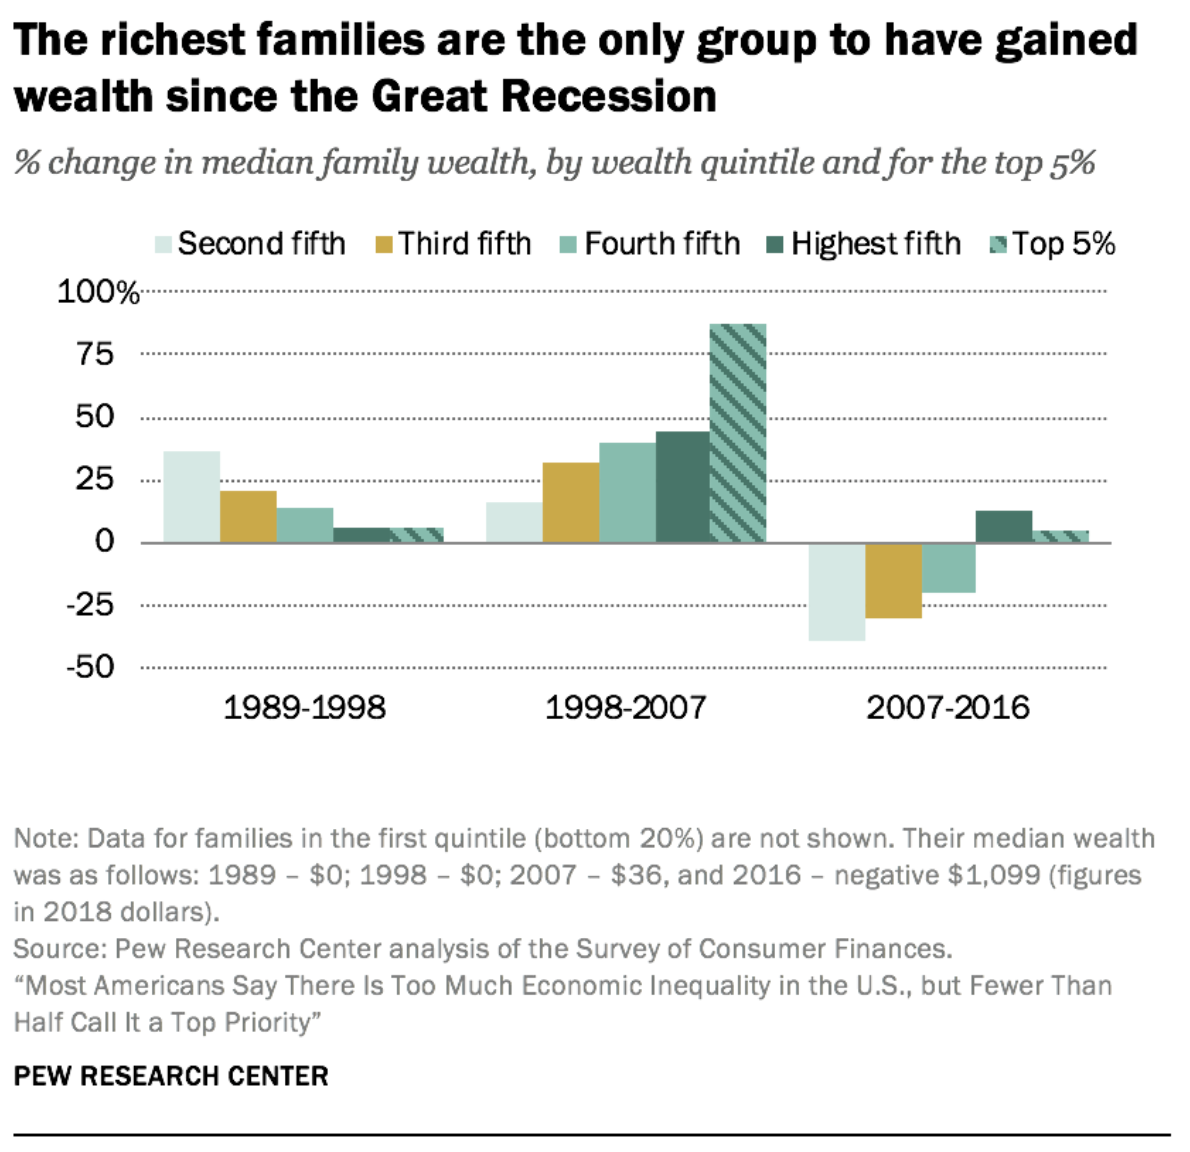
\includegraphics[height = .8\textheight]{pew_wealth}

\end{frame}

\begin{frame}{Class as ownership of capital}{Classic texts}


\includegraphics[width = .4\textwidth]{marx}
\href{https://www.hup.harvard.edu/books/9780674430006}{
\includegraphics[width = .45\textwidth]{piketty}}

\end{frame}

\begin{frame}{Beyond two classes}{Wright, 1997. \bref{https://www-fulcrum-org.proxy.library.cornell.edu/epubs/8c97kt056}{Class Counts}}

For Marx there were two main classes,
\begin{itemize}
\item capitalists (very few)
\item laborers (almost everyone)
\end{itemize}
characterized by conflict and exploitation \vskip .2in
How could we further disaggregate the laborers? \pause
\begin{itemize}
\item authority over others  \pause
\item possession of scarce skills
\end{itemize}

\end{frame}

\begin{frame}{Beyond two classes}{Wright, 1997. \bref{https://www-fulcrum-org.proxy.library.cornell.edu/epubs/8c97kt056}{Class Counts}}

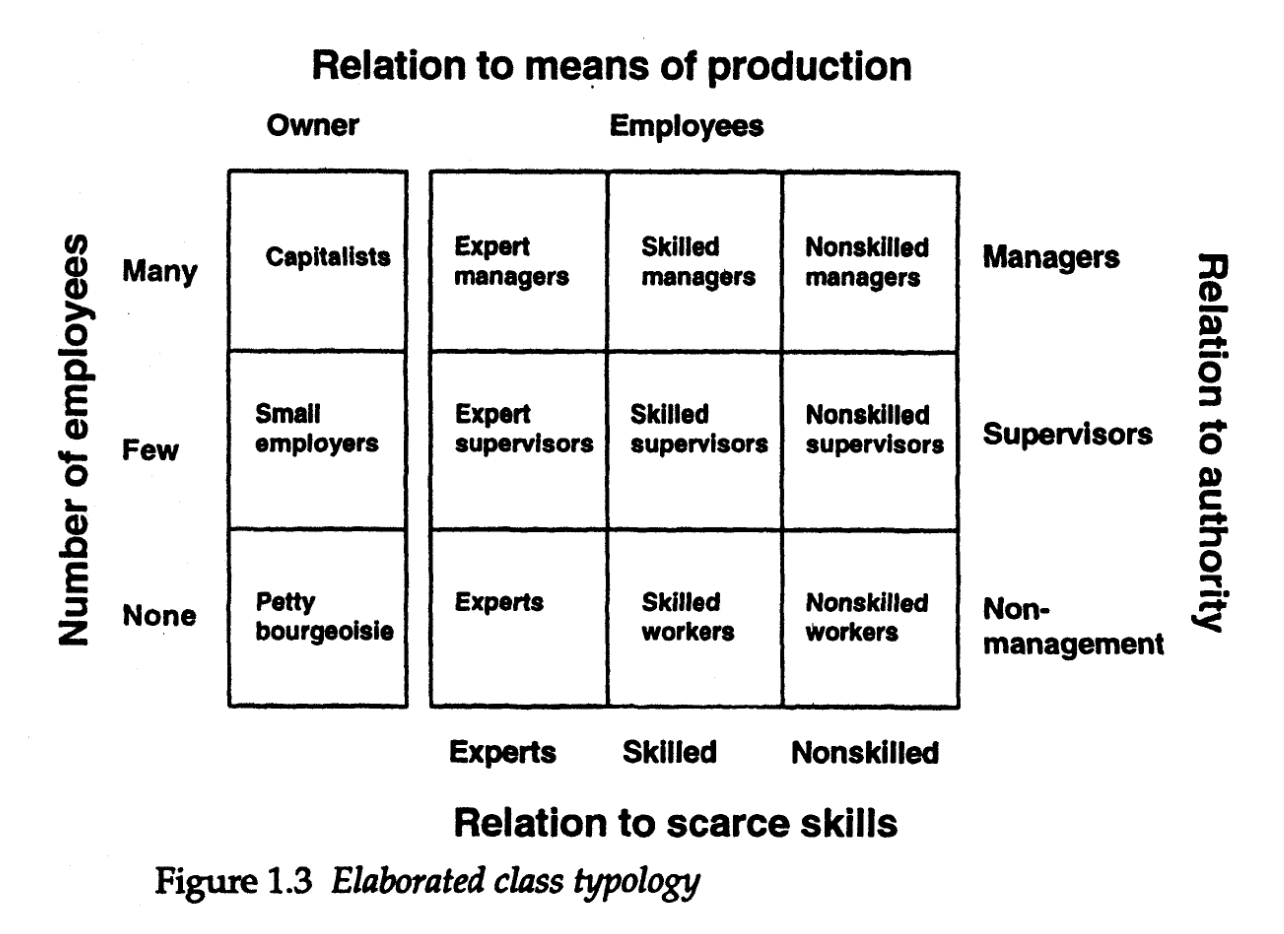
\includegraphics[height = .8\textheight]{wright_classes}

\end{frame}

\begin{frame}{Beyond two classes}

How would you measure classes\\by ownership, authority, and skills? \vskip .2in \pause
\begin{itemize}
\item Categorize jobs into \textbf{occupations}
\begin{itemize}
\item titles based on tasks done at work
\end{itemize}
\item Categorize occupations into classes
\end{itemize}

\end{frame}

\begin{frame}{Beyond two classes}{Erikson, Goldthorpe, \& Portocarero \bref{https://www.jstor.org/stable/589632}{1979}}

\begin{itemize}
\item[I] Higher-grade professionals
\item[II] Lower-grade professionals
\item[III] Routine non-manual
\item[IV] Small proprietors
\item[V/VI] Skilled manual
\item[VII] Unskilled manual
\end{itemize}

\end{frame}

\begin{frame}{Beyond two classes: Class mobility}{From a \bref{https://osf.io/rkw3e}{working paper} with Daniel Molitor and Jennie Brand.\\Data from \bref{https://www.bls.gov/nls/nlsy79.htm}{NLSY79}. Replication code \bref{https://github.com/ilundberg/replication/tree/master/causalmobility}{here}.}

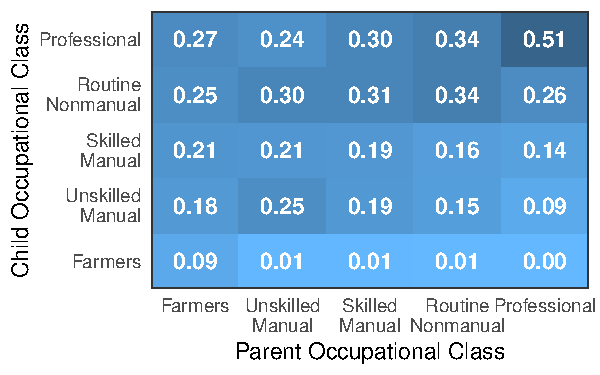
\includegraphics[width = .8\textwidth]{classes_unconditional}

\end{frame}

\begin{frame}{Classes as power relations: A place to go to learn more}

\href{https://www.cambridge.org/core/books/class-counts/E3354F3B204FDFCE9696C2BE5698C959}{
\includegraphics[width = .45\textwidth]{wright}}

\end{frame}

\begin{frame}{Classes and capital that is not financial}{Bourdieu 1986. The Forms of Capital.}

\begin{itemize}
\item<2-> I possess knowledge of data science
\begin{itemize}
\item<5-> \textbf{embodied} cultural capital
\item<6-> \textbf{institutionalized} in educational credentials
\end{itemize} \vskip .1in
\item<3-> Knowledge of data science is highly valued in the economy
\begin{itemize}
\item<7-> value depends on the \textbf{field}
\end{itemize} \vskip .1in
\item<4-> You can buy this knowledge with your tuition
\begin{itemize}
\item<8-> forms of capital are \textbf{fungible}
\end{itemize}
\end{itemize}

\end{frame}

\begin{frame}{Classes and capital that is not financial}{Bourdieu 1986. The Forms of Capital.}

Questions in cultural capital:
\begin{enumerate}
\item what kinds of cultural capital are valued?
\item in what fields?
\item how is that cultural capital acquired?
\end{enumerate}

\end{frame}

\begin{frame}{Classes and capital that is not financial}{Lareau. \bref{https://www.ucpress.edu/book/9780520271425/unequal-childhoods}{Unequal Childhoods.}}

\pause
\begin{itemize}
\item concerted cultivation\pause
\begin{itemize}
\item actively foster skills\pause
\item scheduled activities\pause
\item practiced by middle-class parents
\end{itemize}
\pause
\item accomplishment of natural growth\pause
\begin{itemize}
\item let children grow\pause
\item give them autonomy\pause
\item practiced by working-class parents\pause
\end{itemize}
\end{itemize} \vskip .2in
The field (the U.S. education system and economy)\\rewards concerted cultivation

\end{frame}

\begin{frame}{How could you use data science to study cultural capital?}

One idea: Time diaries
\begin{itemize}
\item PSID-CDS (\bref{https://psidonline.isr.umich.edu/cds/questionnaires/cds-ii/english/cdsiitdday.pdf}{questionnaire})
\item \bref{https://www.atusdata.org/atus-action/time_use_variables/group/3}{American Time Use Study}
\end{itemize}

An example paper: Weininger, Lareau, \& Conley (\bref{https://academic.oup.com/sf/article-abstract/94/2/479/2583788}{2015})

\end{frame}

\begin{frame}{Status}

You are at a party\vskip .2in\pause
``Hi. What do you do?'' \pause
\begin{itemize}
\item A: I'm a medical doctor \pause
\item B: I'm a very skilled gambler \pause
\end{itemize}
Pay might be equal.  \pause These differ in \textbf{status}

\end{frame}

\begin{frame}{Status}

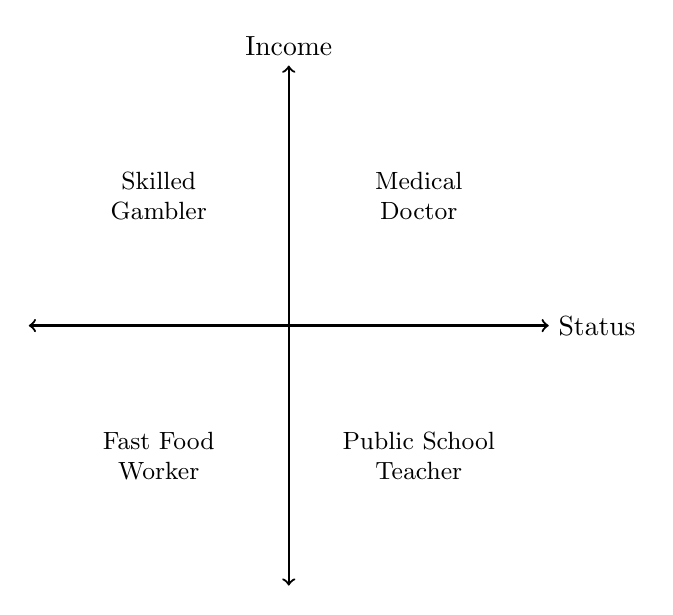
\begin{tikzpicture}[x = 1.3in, y = 1.3in]
\draw[thick, <->] (0,-1) -- (0,1);
\draw[thick, <->] (-1,0) -- (1,0);
\node[anchor = south] at (0,1) {Income};
\node[anchor = west] at (1,0) {Status}; \pause
\node[font = \small, align = center] at (-.5,.5) {Skilled\\Gambler};
\node[font = \small, align = center] at (.5,.5) {Medical\\Doctor}; \pause
\node[font = \small, align = center] at (.5,-.5) {Public School\\Teacher}; \pause
\node[font = \small, align = center] at (-.5,-.5) {Fast Food\\Worker};
\end{tikzpicture}

\end{frame}

\begin{frame}{Status: Measuring with data science}{Example from \bref{https://gss.norc.org/Documents/reports/methodological-reports/MR122\%20Occupational\%20Prestige.pdf}{Smith \& Son 2014}}

Respondents given 90 occupations on paper cards \vskip .2in

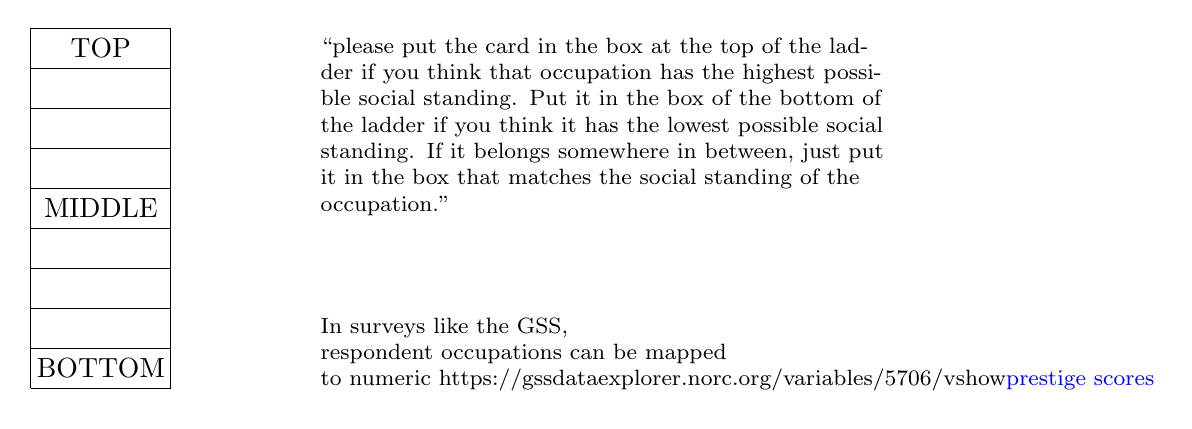
\begin{tikzpicture}[y = .2in, x = .7in]
\draw[ystep = .2in, xstep = .7in] (0,0) grid (1,9);
\node at (.5,8.5) {TOP};
\node at (.5,4.5) {MIDDLE};
\node at (.5,.5) {BOTTOM};
\node[anchor = north west, font = \footnotesize, align = left, text width = .6\textwidth] at (2,9) {``please put the card in the box at the top of the ladder if you think that occupation has the highest possible social standing. Put it in the box of the bottom of the ladder if you think it has the lowest possible social standing. If it belongs somewhere in between, just put it in the box that matches the social standing of the occupation.''};
\node[anchor = north west, align = left, font = \footnotesize] at (2,2) {In surveys like the GSS,\\respondent occupations can be mapped\\to numeric \bref{https://gssdataexplorer.norc.org/variables/5706/vshow}{prestige scores}};
\end{tikzpicture}

\end{frame}

\goalsframe

\end{document}

